%\lipsum[4-4]

This chapter presents the methodology that is intended to be adopted in the development of this PhD thesis. Based on the methodology and expected contributions, a work plan for the upcoming years is presented.

In section \ref{sec:41} is presented an overview of the architecture of proposed work. In sections \ref{sec:42} and \ref{sec:43}, the methodology and expected contributions are detailed. In section \ref{sec:44} is presented the workplan.

\section{Architecture of proposed work}
\label{sec:41}


Framed in this PhD work, a smart metering system can be divided in four major areas, as represented in figure \ref{fig:41topLevel}. On lower level, the needed data is \textbf{measured} (such as voltages, currents and so on). Based on this measurements, \textbf{information} can be obtained (such as power, energy, power factor, GPS location). This information can be stored in databases and, a further step is on the analysis of this information towards obtaining \textbf{knowledge} that can be used in a \textbf{Decision Support System} (DSS).

\begin{figure}[h!]
	\centering
	\vspace{-1em}
	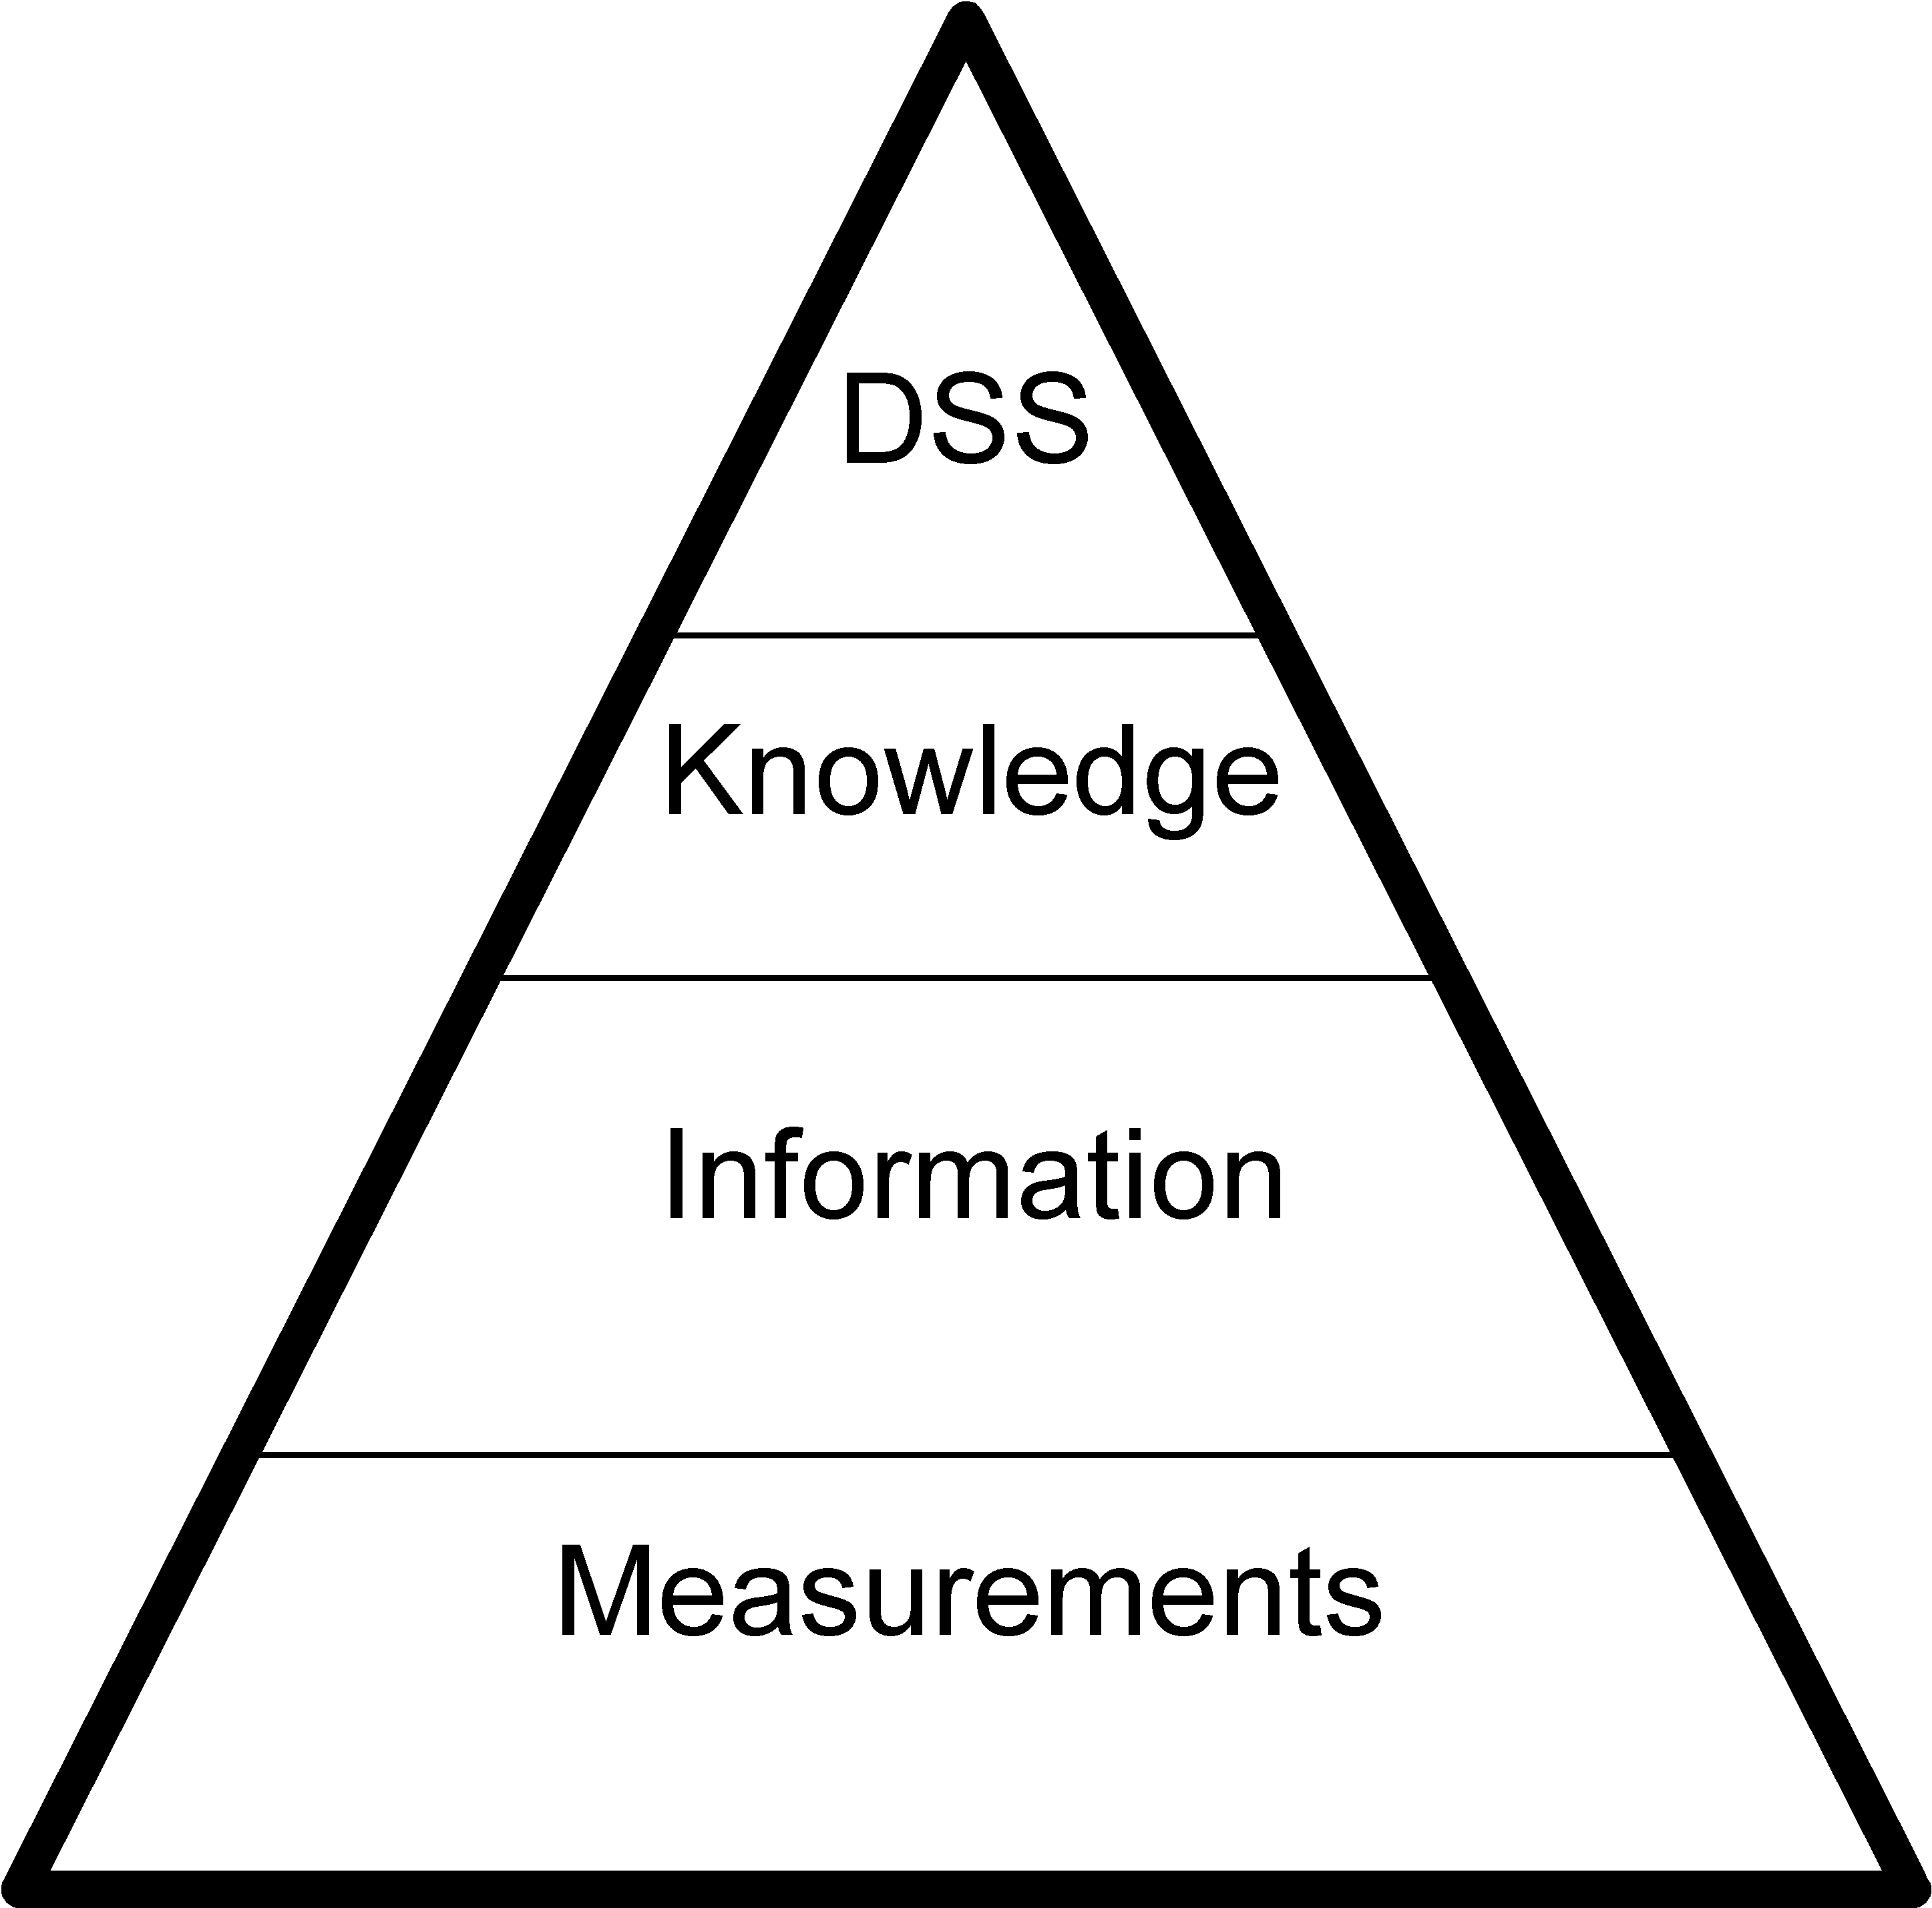
\includegraphics[width=0.3\textwidth,keepaspectratio]{figures/4.Method/pyramid}
	\caption{Overall functional architecture of a smart metering system.}
	\label{fig:41topLevel}
\end{figure}

This work will focus on the first two levels of the smart metering system pyramid. Therefore the energy data must be acquired, processed, transmitted and stored in a centralized database, as represented in figure \ref{fig:41dataFlow}.

\begin{figure}[h!]
	\centering
	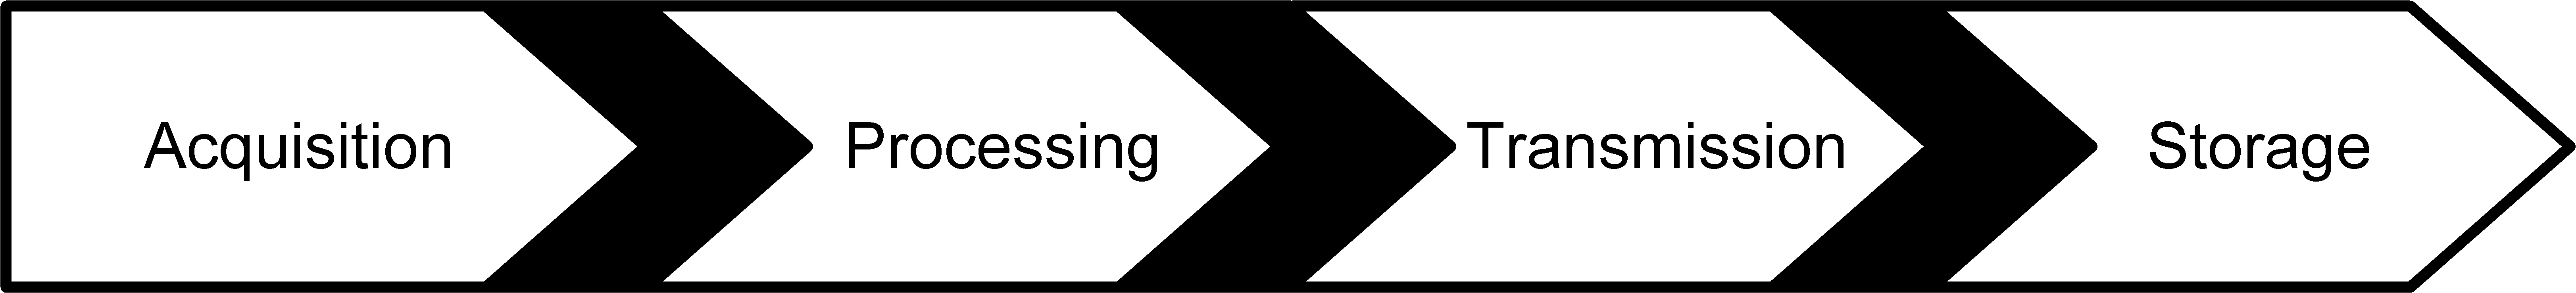
\includegraphics[width=0.8\textwidth,keepaspectratio]{figures/4.Method/data_flow}
	\caption{Data flow of measurement-information layers.}
	\label{fig:41dataFlow}
\end{figure}


For the acquisition part, a non-intrusive self-powered sensor node will be studied. The processing part depends on an accurate knowledge of the catenary and the traction transformer, which depends on train GPS location and power flow conditions. These two parts are further detailed in the methodology and expected contributions of section \ref{sec:42}.

The definition of the processing part will validate if the proposed acquisition architecture has enough support. At this moment a solution with only a current sensor, for the acquisition in each transformer's secondary, is of advanced interest. 

The transmission of the generated information to a centralized storage is further detailed in section \ref{sec:43}. Several models will be considered for accurate simulation of such transmission network. The overall architecture of the system is presented in figure \ref{fig:41architecture}.

\begin{figure}[h!]
	\centering
	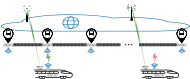
\includegraphics[width=1.0\textwidth,keepaspectratio]{figures/architecture}
	\caption{Architecture of proposed work.}
	\label{fig:41architecture}
\end{figure}







%%%%%%%%%%%%%%%%%%
%%%%%%%%%%%%%%%%%%
%%%%%%%%%%%%%%%%%%
%\newpage
\section{Non-intrusive self-powered sensor node}
\label{sec:42}
\subsection{Purpose}

The purpose of this section is to cover the acquisition and processing parts of the data-flow presented previously. As a starting point, a non-intrusive and self-powered sensor node allows the measurement of AC currents in all transformer secondary windings, as illustrated in figure \ref{fig:4.powerSensing}. This figure is based on the 3400 series train topology of \textit{Comboios de Portugal} (CP) used in urban services.

Based on the field measurements, a data concentrator will receive the current values from each sensor node. This data concentrator generates information based on the estimation of the AC grid voltage and the acquisition of GPS location, as proposed by the European Commission regulation No 1301/2014. For each time-stamp, the active and reactive power is calculated and transmitted together with the geographical position.

In the scope of Shift2Rail, is expected to develop a smart metering system for RTS. Assuming that a non-intrusive measurement system is of extreme interest, this proposal of a non-intrusive and self powered sensor node goes along the goals of Shif2Rail.

On the field of measurement, non-intrusive technical solutions has been used for several years for current measurement, such as hall-effect current sensors, rogowsky probes or current transformers.
For self-powering purposes, some studies on using current transformers for energy harvesting has been proposed <<apresentar papers>>


\begin{figure}[h!]
	\centering
	\vspace{-1em}
	\includegraphics[width=0.7\textwidth,keepaspectratio]{figures/4.Method/powerSensing}
	\caption{Power architecture of case-study train.}
	\label{fig:4.powerSensing}
\end{figure}



\subsection{Contributions}

\begin{itemize}
	\setlength\itemsep{0em}
	\item New energy metering architecture using a non-intrusive approach.
	
	\item Accurate estimation of injected power into catenary, that is needed for train operation, based on on-board measurements.

\end{itemize}


\subsection{Methodology}

The methodology is divided into two parts. The first part will be related to the processing of the data generated by the sensor nodes and the second part is the definition of the sensor itself.

As a starting point of the methodology, it is expected to work on the \textbf{development of models} similar to the ones presented in figure \ref{fig:4.methodElectrical}. The modeling of such architecture allows the evaluation of the power contribution of a train, at a certain instant, to the power injected to the catenary. This methodology will contribute to \textbf{implementation of processing algorithms} in the train data concentrator that, based on the measurement of AC secondary winding's voltages and currents, will generate the accurate value of the energy injected in the catenary by the traction substation. The expected result will be the comparison between the estimation and the measured injected power in the catenary.

In this second part of the methodology, or the acquisition part, the sensor will be defined and validated. As a first step in the methodology, using Ansys or similar Finit Element Method (FEM) software, the \textbf{current and electric field of one winding will be simulated}. With the results of this simulation, the current and voltage sensors will be evaluated. In a further step, \textbf{real experiments on low voltage} will test the proposed sensor node.



\begin{figure}[h!]
	\centering
	\includegraphics[width=0.9\textwidth,keepaspectratio]{figures/4.Method/methodElectrical}
	\caption{Models needed for simulation.}
	\label{fig:4.methodElectrical}
\end{figure}



\subsection{Simulation tools and frameworks}

\cite{pilo2000} identifies the need of two tools for the simulation of railway power lines: (1) the simulator for the railway line and (2) an electrical system simulator. Based on that, \cite{almagro2017} uses the simulation tool \textbf{OpenDSS} with the Python integration for the simulation of the railway power lines. A further study on OpenDSS shows enough documentation and recent updates (march 2017) with the possible integration with VBA Excel, MatLAB and Python scripts.

Mathworks suggests also the usage of \textbf{MatLAB and Simulink} for rail electrical systems modeling. 
Similarly, \textbf{Ansys} products are suggested for the simulation of railway power systems as well as \textbf{PSIM}. The three previously presented products are also flexible to work in co-simulation, with the advantage of choosing the best software for the most straightforward application.

%%%%%%%%%%%%%%%
%%%%%%%%%%%%%%%
%%%%%%%%%%%%%%%

\section{RTS wireless network}
\label{sec:43}

\subsection{Purpose}

The main purpose of the RTS wireless network is to transmit energy measurements and information generated by the nodes to a centralized storage server. 

As a lower level and as previously presented, each train has current sensors as nodes and a data concentrator. Between nodes and data concentrator, AC voltage and current measurements must be exchanged.
At this level, the relevant issue will be the energy consumption of nodes.

Between train data concentrator and ground-level, the train movement should be considered to better comply with the purpose of transmission the information generated at trains to the centralized storage server. 

Further modeling and simulation of a WSN for energy measurement of RTS rolling stock will be made.

\subsection{Contribution}
%An energy measurement system in rolling stock does not require a broadband real-time/continuous communication (such as LTE), being possible to collect and store data in train data concentrator and, while the train is waiting at station for passenger exchange (which lasts for less than one minute), the data is transferred between train and station AP (and then to a remote server). Therefore, the contribution will be the cost reduction of information transmission of energy sensor network data

\begin{itemize}
	\setlength\itemsep{0em}
	
	\item As a starting point, one contribution will be the availability of measured data from trains where currently no energy measurement is performed.
	
	\item A second contribution will be the data-rate increasing of energy measurements, which will result on direct increase on the quality of information of energy.
	
	\item A further contribution can be the avoidance of broadband real-time/continuous communication (such as LTE), being possible to collect and store data in train data concentrator and, while the train is waiting at stations, the data is transferred between train and station AP (and then to a remote server). A possible contribution will be the cost reduction of information transmission of energy sensor network data.
\end{itemize}

\subsection{Methodology}

The methodology for this part will include the \textbf{modeling and simulation} of network blocks similar to the ones presented in figure \ref{fig:4.methodWireless}. An accurate modeling and simulation will define the more appropriate network technologies to implement in this RTS network. 
The simulation will be performed in a NS-3 simulator or similar.
The \textbf{results} of such simulation will define the max data-rate of the sensor nodes as well as the energy consumption required for the information transmission.

\begin{figure}[h!]
	\centering
	\includegraphics[width=0.9\textwidth,keepaspectratio]{figures/4.Method/methodWireless}
	\caption{Models needed for simulation.}
	\label{fig:4.methodWireless}
\end{figure}

\subsection{Simulation tools and frameworks}

Several simulators/emulators were presented in the literature review chapter. From those, special attention is given to the NS-3 simulator and the MatLAB/Simulink tool.  
%<<necessário avaliar melhor os restantes candidatos>>

\section{Work plan}
\label{sec:44}

To be defined.

Secondary tasks of the work plan are the deliverables for the iRail programme and for the FCT institution, which occurs at end of academic year. 


